\chapter{Task and Environment Modelling}\label{chp:environmentTaskModelling}


%===================================================================================================%
\section{Introduction}
%===================================================================================================%

After identifying, specifying, selecting and validating the two system properties \textit{Automated/Limitless Scaling} and \textit{Cost} in chapter~\vref{chp:operationalization}, a task has to be modelled to evaluate a serverless and a non-serverless prototype in chapter~\vref{chp:suitabilityAssessment} and~\vref{chp:viabilityAssessment} respectively. This task serves as a well defined environment and test case for a systematic, explicit, comprehensive and reproducible method of evaluation. 

%===================================================================================================%
\section{Environment Design}
%===================================================================================================%

In order to replicate a real-life use case, various confidential client projects that IBM has been implementing were looked at to derive parameters and to obtain reliable numbers. These numbers will be supported and validated by public available academic sources to maintain the the explicit and reproducible nature of this study.\\
Since the scope of this study is limited to cloud architectures, the environment for the test case will be the to the prototype corresponding cloud environment. For the non-serverless approach, \textit{IBM Cloud}\footnote{\url{https://www.ibm.com/cloud/}} will be used. Likewise, for the serverless approach, \textit{Amazon Web Servives}\footnote{\url{https://aws.amazon.com/}} will be employed. 

\begin{figure}[ht]
    \includegraphics[width=\linewidth]{images/drawio/highlevelTestArch.png}\centering
    \caption{Highlevel Environment Architecture}
    \label{fig:highlevelEnvArch}
\end{figure}

As shown in figure~\vref{fig:highlevelEnvArch}, the environment will consist of a simulated IoT device which represents a sensor that emits messages, a cloud platform and a data processor that is deployed on said cloud platform and will process the messages. The message gateway that receives the message in the first place is implicitly chosen by the choice of cloud platform since it is not in the scope of this study to discuss various gateway solutions and their impact.  \\
After the message is received, it is forwarded to the data processor. To derive tasks (i.e., test cases) from the requirements or system aspects identified, specified, validated and selected in chapter~\vref{chp:operationalization}, parameters within this environment will be introduced in the following two sections. 
    
%******************************************%
\subsection{Automated/Limitless Scaling}\label{ssec:scaling}
%******************************************%

In order to test the scaling capabilities of each proposed architecture, over the time of ten minutes, the amount of messages sent to the system will increase to a maximum of $10,000$ messages per second. This scenario is outlined in~\vref{graph:scalingTask}. Each test round will last $5$ seconds, meaning that at the first test iteration, $10,000$ messages will be sent over the course of $5$ seconds, resulting in $2,000Messages/Second$ ($\dfrac{10,000}{5}=2,000$). Consequently, at the second test iteration, $20,000$ messages will be sent over the course of $5$ seconds, resulting in $4,000Messages/Second$ ($\dfrac{10,000}{5}=4,000$), and so on.\\
After five test iteration the evaluation for the task "Automated/Limitless Scaling" is finished.

\begin{figure}[ht]
    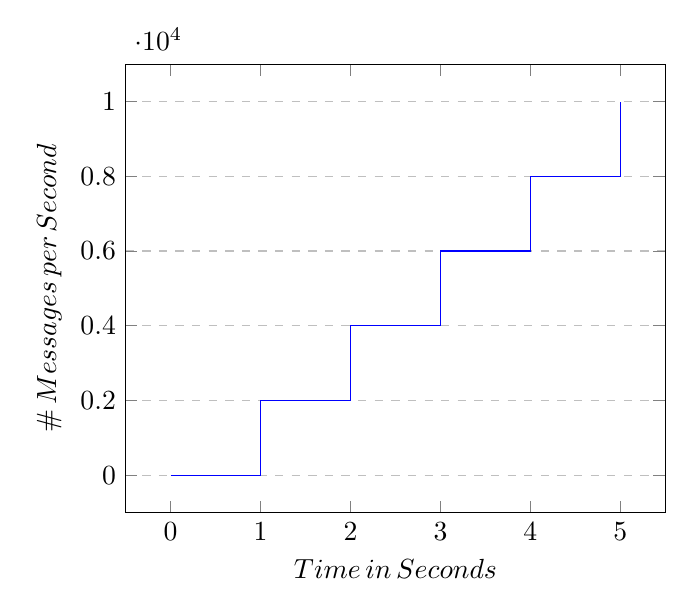
\begin{tikzpicture}
        \begin{axis}[
            xlabel={$Time\,in\,Seconds$},
            ylabel={$\#\,Messages\,per\,Second$},
            % samples=100,
            ymajorgrids=true,
            grid style=dashed,
        ]
        \addplot [const plot, no marks, color=blue] 
            coordinates {(0,0) (1,2000) (2,4000) (3,6000) (4,8000) (5,10000)};
        \end{axis}
    \end{tikzpicture}\centering
    \caption {Automated/Limitless Scaling Task}
    \label{graph:scalingTask}
\end{figure}

The processing task for the data processors will be very simple. Each message will carry a small JSON (JavaScript-Object-Notation) payload to be processed (figure~\vref{fig:messagePayload}). This payload has a size of 61Bytes. Depending on the plaform-specific requirements and recommended practices, the way the payload is sent to the endpoint can differ and is explained in chapter~\vref{chp:prototyping}. 

\begin{figure}
    \begin{lstlisting}[language=json,firstnumber=1]
    {
        "payload": {
            "temp": <int value>
        }
    }
    \end{lstlisting}\centering
    \caption{Message Payload}
    \label{fig:messagePayload}
\end{figure}

To assess how well both prototypes handled the task, the \textit{provisioned compute units} for incoming messages will be compared. 


%******************************************%
\subsection{Cost}
%******************************************%

As for the aspect of scalability, $10,000 Messages\,per\,Second$ will be assumed as the continuous load. To calculate the overall costs for the time-frame of $one\,month$ will be determined. Lower costs are pvreferable.\\
Thevrefore, both prototypes are compared cost-wise for the processing of $10,000 Messages\,per\,Second$.



%===================================================================================================%
\section{Summary}
%===================================================================================================%

The environment will consist of a simulated IoT device which represents a sensor that emits messages, a cloud platform and a data processor that is deployed on said cloud platform and will process the messages. The message gateway that receives the message in the first place is implicitly chosen by the choice of cloud platform. After the message is received, it is forwarded to the data processor.

In order to test the scaling capabilities of each proposed architecture, over the time of ten minutes, the amount of messages sent to the system will increase to a maximum of $10,000$ messages per second. This scenario is outlined in~\vref{graph:scalingTask}. Each test round will last $5$ seconds, meaning that at the first test iteration, $10,000$ messages will be sent over the course of $5$ seconds, resulting in $2,000Messages/Second$ ($\dfrac{10,000}{5}=2,000$).
To assess how well both prototypes scale, the \textit{provisioned compute units} for incoming messages will be compared. 

As for the aspect of scalability, $10,000 Messages\,per\,Second$ will be assumed as the continuous load. To calculate the overall costs for the time-frame of $one\,month$ will be determined. Lower costs are pvreferable.\\
Thevrefore, both prototypes are compared cost-wise for the processing of $10,000 Messages\,per\,Second$ over the course of $one\,month$. 